\documentclass[letterpaper]{article}

\usepackage [english]{babel}
\usepackage [autostyle, english = american]{csquotes}
\MakeOuterQuote{"}
\usepackage{natbib,alifeconf}  %% The order is important
\usepackage{url}
\usepackage{graphicx}
\graphicspath{ {./pictures/} }

\def\imfig#1#2{\begin{figure}[h] \centering \includegraphics[width=\columnwidth]{#1} \caption{#2} \end{figure}}


% *****************
%  Requirements:
% *****************
%
% - All pages sized consistently at 8.5 x 11 inches (US letter size).
% - PDF length <= 8 pages for full papers, <=2 pages for extended
%    abstracts.
% - Abstract length <= 250 words.
% - No visible crop marks.
% - Images at no greater than 300 dpi, scaled at 100%.
% - Embedded open type fonts only.
% - All layers flattened.
% - No attachments.
% - All desired links active in the files.

% Note that the PDF file must not exceed 5 MB if it is to be indexed
% by Google Scholar. Additional information about Google Scholar
% can be found here:
% http://www.google.com/intl/en/scholar/inclusion.html.


% If your system does not generate letter format documents by default,
% you can use the following workflow:
% latex example
% bibtex example
% latex example ; latex example
% dvips -o example.ps -t letterSize example.dvi
% ps2pdf example.ps example.pdf


% For pdflatex users:
% The alifeconf style file loads the "graphicx" package, and
% this may lead some users of pdflatex to experience problems.
% These can be fixed by editing the alifeconf.sty file to specify:
% \usepackage[pdftex]{graphicx}
%   instead of
% \usepackage{graphicx}.
% The PDF output generated by pdflatex should match the required
% specifications and obviously the dvips and ps2pdf steps become
% unnecessary.


% Note:  Some laser printers have a serious problem printing TeX
% output. The use of ps type I fonts should avoid this problem.


\title{They are Very Smart: Genetic-Algorithm-Based Pathfinding in Games}
\author{Joel Tibbetts and Patrick Nuckolls\\
\mbox{}\\
Grinnell College, Grinnell, IA 50112 \\
} % email of corresponding author

% For several authors from the same institution use the same number to
% refer to one address.
%
% If the names do not fit well on one line use
%         Author 1, Author 2 ... \\ {\Large\bf Author n} ...\\ ...
%
% If the title and author information do not fit in the area
% allocated, place \setlength\titlebox{<new height>} after the
% \documentclass line where <new height> is 2.25in


\def\tavs{\textit{They are Very Smart}}
\begin{document}
\maketitle

\begin{abstract}
\tavs~is a destructible tower defense game that explores the viability of short term evolution of neural nets for pathfinding in an adapting adversarial environment.
\end{abstract}

\section{Introduction}
\tavs~is a real-time tower defense game with evolving enemies; which is to say that the player places down towers and other defenses in real time to fend off waves of enemies attempting to destroy the player's "home base." In typical tower defense games, after killing one group of enemies, another comes which is usually stronger than the previous, due to a pre-ordained set of constraints. \tavs~differs from typical tower defense games in that enemy progression is not determined by the game developer, but rather evolves as a result of a genetic algorithm which controls the enemies' damage, movement speed, health, and navigation.

\begin{figure}[h]
	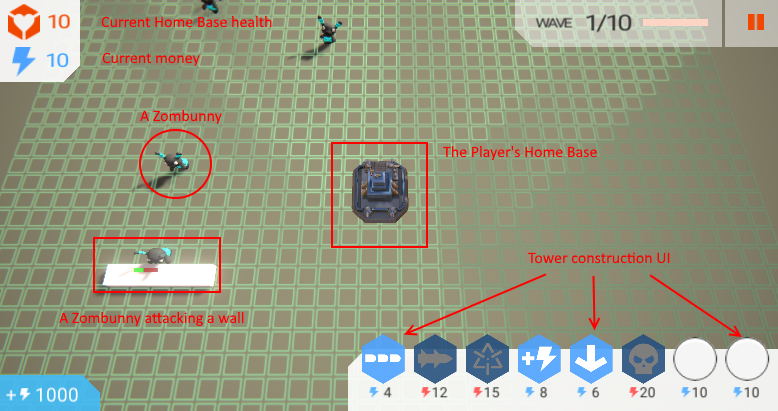
\includegraphics[width=\columnwidth]{InGameLabeled}
	\caption{A screenshot from the game, with various elements labeled}
\end{figure}

In \tavs, player interaction consists of constructing defenses around a central home base. The home base exists in a fixed location in the center of the map, has a set maximum health, and can be damaged by attacks from enemies. Waves of enemies will spawn indefinitely and attempt to destroy the home base. When the health of the home base reaches zero, the game ends.

Players begin the game with an initial sum of money, which can be used to purchase defenses from the tower construction UI (see Figure 1). Defenses are damageable structures which the player may place on any unoccupied square within the defense placement grid.
\imfig{ZoomedOut}{The initial state of the game, showing the home base in the middle of the defense placement grid}

Defenses provide various benefits to the player, such as physically blocking the path of enemies or actively damaging enemies with projectile-based attacks. Some examples of defenses include:
\begin{itemize}
	\item Walls (vertical/horizontal) - inexpensive defenses which block the path of enemies
	\item Machine gun turrets - towers which fire damaging projectiles at nearby enemies
	\item Energy pylons - fragile towers which deal no damage, but instead passively generate income for the player
\end{itemize}

Defenses cost money, which may be gained by killing attacking enemies. As the game progresses, the player may fortify their base by purchasing more expensive defenses and designing complex arrangements of walls and towers in order to thwart enemies.

\pagebreak
In \tavs, the player must defend their home base against the aforementioned onslaught of enemies such as the fearsome Zombunny (see Figure 3). Zombunnies are driven by a single goal: destruction of the player's home base. Zombunnies spawn in groups of ten (separated by a slight delay) at the beginning of the game. Subsequent waves spawn after all members from the previous wave have died. Zombunnies use a genetic algorithm in conjunction with a recurrent neural network to evolve a pathfinding algorithm between generations (waves), with the long-term incentive of dealing damage to the player's base (explain fitness criteria more concisely here). Zombunnies can be killed by either taking damage from a player's defenses or through "starvation." A Zombunny will starve to death if it does not take or deal damage for a given length of time. Through this starvation mechanism, the Zombunnies which survive the longest are ultimately those which interact the most with the player's defenses, and are subsequently more likely to pass on attributes of their genome to the next generation. Zombunnies have three characteristic attributes: health, damage, and movement speed. All three of these stats are assigned upon spawning as dictated by their genome. Pathfinding is controlled by a recurrent neural net, whose weights are determined through a genetic algorithm between waves, which optimizes for Zombunnies' ability to achieve their overarching goal of player base destruction. Zombunnies can "see" nearby entities within a certain radius, including other Zombunnies, player defenses, and the player's home base (when in range). Based on the combination of visible inputs, Zombunnies will output a chosen direction which they will then walk in. This algorithm updates on a tick-by-tick basis. Zombunnies will damage structures they collide with. Because evolution of the pathfinding neural net only happens between generations, near the beginning of the game, Zombunnies will start off with relatively stupid pathfinding which will typically cause the first few populations to starve to death without dealing any significant damage. This provides the player with an initial grace period during which they may build their initial defenses. As time goes on, Zombunnies will evolve towards an optimal stat distribution of health, damage, and speed, as well as in their ability to pathfind in such a way as to thwart the player's defenses and end the game.

\imfig{ZombunnyColliders}{A Zombunny, with attacker and damage colliders highlighted}

%overview
%\begin{itemize}
%    \item Description of tower-defense UI
%    \item Placement of walls vs. towers
%    \item "Spawn points" for zombies
%    \item Central defensible location
%    \item Economy
%    \item Game end/lack thereof
%\end{itemize}

\tavs~was initially inspired by Numantian Games' \textit{They Are Billions}, a game in which a player must build defenses in order to fend off a zombie apocalypse. The game features massive numbers of zombies. This project emerged from an interest in what \textit{They Are Billions} would be like if the zombies could actually think for themselves. The result is significantly pared down in comparison, as the focus has been on zombie evolution as opposed to player interactivity and enjoyability. However, similarities to \textit{They Are Billions} can be seen in the resource management system, the player's defense of a citadel, and need to fend off the faceless hordes. In contrast, \textit{They Are Billions} puts additional emphasis on world generation, player exploration, and narrative elements.

Insert picture of \textit{They Are Billions} gameplay here.

\section{Background}
In \tavs, we utilize a basic genetic algorithm to train a recurrent neural network generated using the Neuroevolution of Augmenting Topologies (NEAT) method, ~cite http://sharpneat.sourceforge.net/~ with https://www.heatonresearch.com/encog/, which is a generalized deep-learning library that includes implementations of NEAT and HyperNEAT.

NEAT is particularly applicable to our issue because it allows the evolution of different topologies and weights in neural networks at the same time, unlike standard back-propagation learning, and is also well-suited for encoding into a genome for evolution. NEAT works by encoding a function that then generates a neural net (citation needed), starting out with low complexity of topology, which can then evolve towards more complex topologies.

Insert helpful diagram here




\section{Tutorial}

\subsection{Running the game}
Our game can be found at
\href{https://github.com/YourFin/They-Are-Very-Smart}{github.com/yourfin/They-Are-Very-Smart},
and downloaded with a standard \texttt{git clone} command. The relevant unity
scene is then located at
\url{They-Are-Very-Smart/TD/TowerDefence/Assets/Scenes/Levels/Level0/Level0.unity}
Double clicking on this file on any computer with unity installed will open up
the unity editor with the context for this paper.

Overview
\begin{itemize}
    \item Unity
    \item Tower Defense tutorial
    \item Action Game Framework
    \item Creating custom towers
    \item Custom scripts
        \begin{itemize}
            \item Genome
            \item ZombieAgent
            \item GenomeManager
            \item ZombieAttacker
        \end{itemize}
    \item Problems importing packages
    \item Relevant parts of Encog framework
        \begin{itemize}
            \item Manually pulling out Encog training methods for neural nets
            \item Stealing Softmax function
        \end{itemize}
    \item Point array stats system
    \item Details of genetic algorithm
        \begin{itemize}
            \item Mutation
            \item Keeping track of fitness
            \item Population management
            \item Starvation function
        \end{itemize}
\end{itemize}


\section{Preliminary Results and Discussion}
Over the course of this project, we learned more about game design than we did
evolutionary algorithms and artificial life. The majority of our time working on
this project was spent dealing with learning the basics of Unity and C\#, which
presented a very significant challenge that we vastly underestimated.

At this time, we are waiting on actual results from our project.
We hope that given a large enough population of zombies, we might see
populations of zombies evolving to counteract players' strategies. Evolution
will likely have little trouble tackling a trivial or consistent player
strategy, like rebuilding the same towers in the same place and
relying heavily on a single tower type, but may have trouble keeping
up with a player that constantly changes strategy over the course of the game.
Our system of softmaxing the genome speed, health, and damage could also
result in progressively larger values relative to the mutation rate, making it
hard for long-evolved high speed value to be traded for damage in the face of
changing player strategies.

Zombunnies will likely evolve around quirks in the way the
game is organized. The primary example would be having health that is just above
multiples of tower damage, allowing it to sustain an additional hit with
insignificant investment in the health stat. This particular problem could be
solved by having towers deal damage with slight randomness, but there likely
exist similar problems that have not been considered.

Players, on the other hand, may also learn to optimize around our implementation
of evolution. Conceivably clever player could develop two very different
strategies ahead of time. The player would first implement the weaker strategy,
and as soon as the zombunnies have deeply rooted themselves in the local maximum
versus that strategy, the strategy could be changed to the second strategy,
leaving the zombunnies unable to easily adapt to the new strategy.

Solving these problems would probably involve moving towards more complicated
models of selection and reproduction than our current keep \(n\) percent,
asexually reproduce the best genomes and then do a straight pass of mutation.
Moving to a system where reproductive resources are distributed according to the
Z-score (standard deviations from the mean) or similar of fitness that give more
reproductive power to individual that more drastically improve on the status quo
could allow for a system that reacts more strongly to change. Another option
could be coding part of the mutation rate in genomes to allow evolution to
determine it's own speed. The two previous approaches could even be combined for
as dynamic an evolution environment as possible.

Sexual (genderless) reproduction could also be introduced as a way of trying to
increase diversity. Plain sexual reproduction without any further restrictions
could allow good traits that evolve in parallel to be combined into a single
individual with the benefits of both, which has fairly obvious advantages.
This simple approach to sexual reproduction could, however, force a single
species to dominate quickly depending on how well neural net parameters combine,
as it could easily be the case that two disparately evolving neural nets combine
into a total dud, despite having fit parents. One way around that would be to
condition reproduction on similarity, such genomes are more likely to reproduce
with those that are structurally similar. Another approach would be to allow
genomes to determine mating preference based on other genomes' content and
fitness, and then run them through a tournament to determine mates. This would
have the additional benefit of allowing additional emergent behavior that has
not been conceived of in this speculation.

Conceptually, evolving neural nets instead of using backpropagation
has the massive benefit of not worrying about how to differentiate and nicely
back-propagate the reward/fitness function to learn, which opens up the
possibility to drop in a nerual net to replace any function in a learning
environment; on a larger timescale, the selection tournament process itself
could modeled with a recurrent neural network, and evolved over multiple plays
of the game.

Allowing the zombunnies to keep track of what they learn from game to game could
be useful as a ``hard mode'' should the base game be too easy, perhaps with the
additional information passed to the navigation function of the round. In an actual game
using this technology to evolve AI, this could be expanded to the entire
playerbase training a single pathfinding algorithm that is then redistributed to
each client, and perhaps even takes in all previous player game history as
additional input. The missing backpropagation requirement opens up
any function to becoming an neural net, and with any input.

\section{Conclusion}
\begin{itemize}
    \item Synopsis of project
    \item Future work and next steps
\end{itemize}

\section{Acknowledgments}
\begin{itemize}
    \item Use of multiple tutorials/repositories
    \begin{itemize}
        \item Encog Machine Learning Framework
        \item Unity Tower Defense Tutorial
        \item Unity Action Game Shooter Tutorial
        \item Redzen repository for normal random numbers
        \item
    \end{itemize}
\end{itemize}

\footnotesize
\bibliographystyle{apalike}
\bibliography{bibliography} % replace by the name of your .bib file

\end{document}
